\documentclass[letterpaper]{article} % DO NOT CHANGE THIS
\usepackage[submission]{aaai2027}  % DO NOT CHANGE THIS
\usepackage[hyphens]{url}  % DO NOT CHANGE THIS
\usepackage{graphicx} % DO NOT CHANGE THIS
\urlstyle{rm} % DO NOT CHANGE THIS
\def\UrlFont{\rm}  % DO NOT CHANGE THIS
\usepackage{natbib}  % DO NOT CHANGE THIS AND DO NOT ADD ANY OPTIONS TO IT
\usepackage{caption} % DO NOT CHANGE THIS AND DO NOT ADD ANY OPTIONS TO IT
\frenchspacing  % DO NOT CHANGE THIS
\usepackage{booktabs}
\pdfinfo{
/TemplateVersion (2027.1)
}
% Official AAAI-27 author kit (https://aaai.org/authorkit27/, AuthorKit27.zip, sha256 9406a545...c960):
% aaai2027.sty and aaai2027.bst copied unchanged; preamble lines above taken from AnonymousSubmission2027.tex.
\setcounter{secnumdepth}{1} % the kit allows 1 or 2 when section numbers are wanted

% Every number comes from here (generated by scripts/cale/paper_numbers.py). Never type a number by hand.
% TODO before submission: the kit requires a single source file, so paste numbers.tex and the \input tables inline.
% Generated by scripts/cale/paper_numbers.py from paper/cale/numbers.json. Do not edit by hand.
% Percent macros hold the number only; write \QuietCVReduction\% in the text. <Name>CI holds the 95% interval.
\newcommand{\QuietTestHints}{1.22}% locked-test: test.quiet.hints
\newcommand{\QuietTestHintsCI}{[1.04, 1.41]}
\newcommand{\QuietTestReduction}{52.0}% locked-test: test.quiet.reduction
\newcommand{\QuietTestMissed}{3.7}% locked-test: test.quiet.missed
\newcommand{\QuietTestMissedCI}{[2.2, 5.3]}
\newcommand{\QuietTestMissedN}{19}% locked-test: test.quiet.missed_n
\newcommand{\QuietCVHints}{1.31}% CV: cv.quiet.hints
\newcommand{\QuietCVHintsCI}{[1.22, 1.42]}
\newcommand{\QuietCVReduction}{50.7}% CV: cv.quiet.reduction
\newcommand{\QuietCVReductionCI}{[49.0, 52.2]}
\newcommand{\QuietCVMissed}{6.2}% CV: cv.quiet.missed
\newcommand{\QuietCVMissedCI}{[5.3, 7.2]}
\newcommand{\QuietCVMissedN}{142}% CV: cv.quiet.missed_n
\newcommand{\BalancedTestHints}{2.15}% locked-test: test.balanced.hints
\newcommand{\BalancedTestHintsCI}{[1.86, 2.47]}
\newcommand{\BalancedTestReduction}{15.1}% locked-test: test.balanced.reduction
\newcommand{\BalancedTestMissed}{0.2}% locked-test: test.balanced.missed
\newcommand{\BalancedTestMissedCI}{[0.0, 0.6]}
\newcommand{\BalancedTestMissedN}{1}% locked-test: test.balanced.missed_n
\newcommand{\BalancedCVHints}{2.32}% CV: cv.balanced.hints
\newcommand{\BalancedCVHintsCI}{[2.16, 2.50]}
\newcommand{\BalancedCVReduction}{12.8}% CV: cv.balanced.reduction
\newcommand{\BalancedCVReductionCI}{[11.8, 13.8]}
\newcommand{\BalancedCVMissed}{0.3}% CV: cv.balanced.missed
\newcommand{\BalancedCVMissedCI}{[0.1, 0.5]}
\newcommand{\BalancedCVMissedN}{6}% CV: cv.balanced.missed_n
\newcommand{\SupportiveTestHints}{2.46}% locked-test: test.supportive.hints
\newcommand{\SupportiveTestHintsCI}{[2.14, 2.79]}
\newcommand{\SupportiveTestReduction}{3.2}% locked-test: test.supportive.reduction
\newcommand{\SupportiveTestMissed}{0.0}% locked-test: test.supportive.missed
\newcommand{\SupportiveTestMissedCI}{[0.0, 0.0]}
\newcommand{\SupportiveTestMissedN}{0}% locked-test: test.supportive.missed_n
\newcommand{\SupportiveCVHints}{2.59}% CV: cv.supportive.hints
\newcommand{\SupportiveCVHintsCI}{[2.41, 2.79]}
\newcommand{\SupportiveCVReduction}{2.8}% CV: cv.supportive.reduction
\newcommand{\SupportiveCVReductionCI}{[2.4, 3.3]}
\newcommand{\SupportiveCVMissed}{0.0}% CV: cv.supportive.missed
\newcommand{\SupportiveCVMissedCI}{[0.0, 0.1]}
\newcommand{\SupportiveCVMissedN}{1}% CV: cv.supportive.missed_n
\newcommand{\AlwaysHelpTestHints}{2.54}% locked-test: test.always_help.hints
\newcommand{\AlwaysHelpTestHintsCI}{[2.20, 2.89]}
\newcommand{\AlwaysHelpTestReduction}{0.0}% locked-test: test.always_help.reduction
\newcommand{\AlwaysHelpTestMissed}{0.0}% locked-test: test.always_help.missed
\newcommand{\AlwaysHelpTestMissedCI}{[0.0, 0.0]}
\newcommand{\AlwaysHelpTestMissedN}{0}% locked-test: test.always_help.missed_n
\newcommand{\AlwaysHelpCVHints}{2.67}% CV: cv.always_help.hints
\newcommand{\AlwaysHelpCVHintsCI}{[2.49, 2.87]}
\newcommand{\AlwaysHelpCVReduction}{0.0}% CV: cv.always_help.reduction
\newcommand{\AlwaysHelpCVReductionCI}{[0.0, 0.0]}
\newcommand{\AlwaysHelpCVMissed}{0.0}% CV: cv.always_help.missed
\newcommand{\AlwaysHelpCVMissedCI}{[0.0, 0.0]}
\newcommand{\AlwaysHelpCVMissedN}{0}% CV: cv.always_help.missed_n
\newcommand{\TwoWrongTestHints}{1.28}% locked-test: test.two_wrong.hints
\newcommand{\TwoWrongTestHintsCI}{[1.09, 1.47]}
\newcommand{\TwoWrongTestReduction}{49.7}% locked-test: test.two_wrong.reduction
\newcommand{\TwoWrongTestMissed}{25.9}% locked-test: test.two_wrong.missed
\newcommand{\TwoWrongTestMissedCI}{[21.5, 30.0]}
\newcommand{\TwoWrongTestMissedN}{134}% locked-test: test.two_wrong.missed_n
\newcommand{\TwoWrongCVHints}{1.38}% CV: cv.two_wrong.hints
\newcommand{\TwoWrongCVHintsCI}{[1.27, 1.50]}
\newcommand{\TwoWrongCVReduction}{48.3}% CV: cv.two_wrong.reduction
\newcommand{\TwoWrongCVReductionCI}{[46.8, 49.7]}
\newcommand{\TwoWrongCVMissed}{27.3}% CV: cv.two_wrong.missed
\newcommand{\TwoWrongCVMissedCI}{[25.4, 29.3]}
\newcommand{\TwoWrongCVMissedN}{622}% CV: cv.two_wrong.missed_n
\newcommand{\ThreeWrongTestHints}{0.70}% locked-test: test.three_wrong.hints
\newcommand{\ThreeWrongTestHintsCI}{[0.59, 0.84]}
\newcommand{\ThreeWrongTestReduction}{72.4}% locked-test: test.three_wrong.reduction
\newcommand{\ThreeWrongTestMissed}{56.6}% locked-test: test.three_wrong.missed
\newcommand{\ThreeWrongTestMissedCI}{[52.0, 61.1]}
\newcommand{\ThreeWrongTestMissedN}{293}% locked-test: test.three_wrong.missed_n
\newcommand{\ThreeWrongCVHints}{0.75}% CV: cv.three_wrong.hints
\newcommand{\ThreeWrongCVHintsCI}{[0.68, 0.81]}
\newcommand{\ThreeWrongCVReduction}{72.0}% CV: cv.three_wrong.reduction
\newcommand{\ThreeWrongCVReductionCI}{[70.6, 73.3]}
\newcommand{\ThreeWrongCVMissed}{57.6}% CV: cv.three_wrong.missed
\newcommand{\ThreeWrongCVMissedCI}{[55.4, 59.7]}
\newcommand{\ThreeWrongCVMissedN}{1{,}312}% CV: cv.three_wrong.missed_n
\newcommand{\RandomTestHints}{1.22}% locked-test: test.random.hints
\newcommand{\RandomTestHintsCI}{[1.06, 1.39]}
\newcommand{\RandomTestReduction}{52.0}% locked-test: test.random.reduction
\newcommand{\RandomTestMissed}{33.2}% locked-test: test.random.missed
\newcommand{\RandomTestMissedCI}{[31.4, 34.7]}
\newcommand{\RandomTestMissedN}{171}% locked-test: test.random.missed_n
\newcommand{\RandomCVHints}{1.31}% CV: cv.random.hints
\newcommand{\RandomCVHintsCI}{[1.22, 1.42]}
\newcommand{\RandomCVReduction}{50.7}% CV: cv.random.reduction
\newcommand{\RandomCVReductionCI}{[50.0, 51.3]}
\newcommand{\RandomCVMissed}{33.2}% CV: cv.random.missed
\newcommand{\RandomCVMissedCI}{[32.4, 34.0]}
\newcommand{\RandomCVMissedN}{757}% CV: cv.random.missed_n
\newcommand{\PFATestHints}{1.44}% locked-test: test.pfa.hints
\newcommand{\PFATestHintsCI}{[1.23, 1.66]}
\newcommand{\PFATestReduction}{43.2}% locked-test: test.pfa.reduction
\newcommand{\PFATestMissed}{2.1}% locked-test: test.pfa.missed
\newcommand{\PFATestMissedCI}{[0.9, 3.6]}
\newcommand{\PFATestMissedN}{11}% locked-test: test.pfa.missed_n
\newcommand{\PFACVHints}{1.56}% CV: cv.pfa.hints
\newcommand{\PFACVHintsCI}{[1.45, 1.69]}
\newcommand{\PFACVReduction}{41.3}% CV: cv.pfa.reduction
\newcommand{\PFACVReductionCI}{[39.8, 42.7]}
\newcommand{\PFACVMissed}{3.6}% CV: cv.pfa.missed
\newcommand{\PFACVMissedCI}{[2.8, 4.5]}
\newcommand{\PFACVMissedN}{83}% CV: cv.pfa.missed_n
\newcommand{\RiskHeadTestHints}{1.30}% locked-test: test.risk_head.hints
\newcommand{\RiskHeadTestHintsCI}{[1.10, 1.50]}
\newcommand{\RiskHeadTestReduction}{48.8}% locked-test: test.risk_head.reduction
\newcommand{\RiskHeadTestMissed}{2.9}% locked-test: test.risk_head.missed
\newcommand{\RiskHeadTestMissedCI}{[1.5, 4.3]}
\newcommand{\RiskHeadTestMissedN}{15}% locked-test: test.risk_head.missed_n
\newcommand{\RiskHeadCVHints}{1.42}% CV: cv.risk_head.hints
\newcommand{\RiskHeadCVHintsCI}{[1.31, 1.54]}
\newcommand{\RiskHeadCVReduction}{46.7}% CV: cv.risk_head.reduction
\newcommand{\RiskHeadCVReductionCI}{[45.1, 48.5]}
\newcommand{\RiskHeadCVMissed}{3.8}% CV: cv.risk_head.missed
\newcommand{\RiskHeadCVMissedCI}{[3.0, 4.6]}
\newcommand{\RiskHeadCVMissedN}{86}% CV: cv.risk_head.missed_n
\newcommand{\TestStudents}{597}% locked-test: test.n_students
\newcommand{\TestSequences}{3{,}468}% locked-test: test.n_sequences
\newcommand{\TestStuck}{570}% locked-test: test.n_stuck
\newcommand{\TestStuckOpp}{518}% locked-test: test.n_stuck_opp
\newcommand{\QuietTestJDiffAH}{-2.196}% locked-test: test.quiet.jdiff_ah
\newcommand{\QuietTestJDiffAHCI}{[-2.679, -1.750]}
\newcommand{\BalancedTestJDiffAH}{-0.236}% locked-test: test.balanced.jdiff_ah
\newcommand{\BalancedTestJDiffAHCI}{[-0.310, -0.161]}
\newcommand{\SupportiveTestJDiffAH}{-0.025}% locked-test: test.supportive.jdiff_ah
\newcommand{\SupportiveTestJDiffAHCI}{[-0.079, 0.052]}
\newcommand{\QuietTestJDiffTwoWrong}{-0.913}% locked-test: test.quiet.jdiff_two_wrong
\newcommand{\QuietTestJDiffTwoWrongCI}{[-1.193, -0.643]}
\newcommand{\QuietValHints}{1.35}% validation: val.quiet.hints
\newcommand{\AlwaysHelpValHints}{2.70}% validation: val.always_help.hints
\newcommand{\QuietValMissed}{4.8}% validation: val.quiet.missed
\newcommand{\QuietValReduction}{49.8}% validation: val.quiet.reduction
\newcommand{\BKTValAUCA}{0.813}% validation: val.bkt_auc_k3
\newcommand{\BKTValAUCACI}{[0.794, 0.833]}
\newcommand{\BKTValAUCB}{0.805}% validation: val.bkt_auc_k5
\newcommand{\BKTValAUCBCI}{[0.784, 0.828]}
\newcommand{\BKTValAUCC}{0.911}% validation: val.bkt_auc_k8
\newcommand{\BKTValAUCCCI}{[0.888, 0.931]}
\newcommand{\DKTMinusBKTAUCA}{-0.003}% validation: val.dkt_minus_bkt_k3
\newcommand{\DKTMinusBKTAUCACI}{[-0.010, 0.004]}
\newcommand{\DKTMinusBKTAUCB}{-0.003}% validation: val.dkt_minus_bkt_k5
\newcommand{\DKTMinusBKTAUCBCI}{[-0.010, 0.004]}
\newcommand{\SAKTMinusBKTAUCA}{-0.008}% validation: val.sakt_minus_bkt_k3
\newcommand{\SAKTMinusBKTAUCACI}{[-0.015, -0.000]}
\newcommand{\SAKTMinusBKTAUCB}{-0.013}% validation: val.sakt_minus_bkt_k5
\newcommand{\SAKTMinusBKTAUCBCI}{[-0.022, -0.005]}
\newcommand{\DKTPromoted}{no}% validation: val.dkt_promoted
\newcommand{\SAKTPromoted}{no}% validation: val.sakt_promoted
\newcommand{\MSDKTMinusBKTAUCA}{-0.004}% validation: val.ms_dkt_minus_bkt_k3
\newcommand{\MSDKTMinusBKTAUCACI}{[-0.017, 0.008]}
\newcommand{\MSDKTMinusBKTAUCB}{-0.010}% validation: val.ms_dkt_minus_bkt_k5
\newcommand{\MSDKTMinusBKTAUCBCI}{[-0.022, 0.003]}
\newcommand{\MSDKTPromoted}{no}% validation: val.ms_dkt_promoted
\newcommand{\MSSAKTMinusBKTAUCA}{-0.011}% validation: val.ms_sakt_minus_bkt_k3
\newcommand{\MSSAKTMinusBKTAUCACI}{[-0.026, 0.004]}
\newcommand{\MSSAKTMinusBKTAUCB}{-0.008}% validation: val.ms_sakt_minus_bkt_k5
\newcommand{\MSSAKTMinusBKTAUCBCI}{[-0.023, 0.008]}
\newcommand{\MSSAKTPromoted}{no}% validation: val.ms_sakt_promoted
\newcommand{\CVStudents}{2{,}349}% CV: cv.n_students
\newcommand{\CVSequences}{14{,}640}% CV: cv.n_sequences
\newcommand{\CVStuckOpp}{2{,}279}% CV: cv.n_stuck_opp
\newcommand{\AsevenQuietDThreeReduction}{50.1}% CV: a7.D3.quiet.reduction
\newcommand{\AsevenQuietDThreeReductionCI}{[48.5, 51.6]}
\newcommand{\AsevenQuietDThreeMissed}{6.2}% CV: a7.D3.quiet.missed
\newcommand{\AsevenQuietDThreeMissedCI}{[5.2, 7.2]}
\newcommand{\AsevenQuietDFourReduction}{8.3}% CV: a7.D4.quiet.reduction
\newcommand{\AsevenQuietDFourReductionCI}{[7.5, 9.2]}
\newcommand{\AsevenQuietDFourMissed}{0.2}% CV: a7.D4.quiet.missed
\newcommand{\AsevenQuietDFourMissedCI}{[0.1, 0.3]}
\newcommand{\AsevenQuietDFiveTFifteenReduction}{26.4}% CV: a7.D5T15.quiet.reduction
\newcommand{\AsevenQuietDFiveTFifteenReductionCI}{[24.7, 28.2]}
\newcommand{\AsevenQuietDFiveTFifteenMissed}{4.3}% CV: a7.D5T15.quiet.missed
\newcommand{\AsevenQuietDFiveTFifteenMissedCI}{[3.4, 5.3]}
\newcommand{\AsevenQuietDFiveTTwentyReduction}{41.6}% CV: a7.D5T20.quiet.reduction
\newcommand{\AsevenQuietDFiveTTwentyReductionCI}{[39.2, 43.8]}
\newcommand{\AsevenQuietDFiveTTwentyMissed}{10.4}% CV: a7.D5T20.quiet.missed
\newcommand{\AsevenQuietDFiveTTwentyMissedCI}{[8.1, 12.7]}
\newcommand{\AsevenQuietDEmaReduction}{7.1}% CV: a7.DEMA.quiet.reduction
\newcommand{\AsevenQuietDEmaReductionCI}{[6.2, 8.0]}
\newcommand{\AsevenQuietDEmaMissed}{0.3}% CV: a7.DEMA.quiet.missed
\newcommand{\AsevenQuietDEmaMissedCI}{[0.2, 0.5]}
\newcommand{\AsevenQuietTauMin}{0.51}% CV: a7.D3.quiet.tau_min
\newcommand{\AsevenQuietTauMax}{0.60}% CV: a7.D3.quiet.tau_max
\newcommand{\AsixSimQuietBeats}{40}% exploratory: a6.quiet.beats
\newcommand{\AsixSimQuietTies}{5}% exploratory: a6.quiet.indistinguishable
\newcommand{\AsixSimQuietFlips}{55}% exploratory: a6.quiet.flips
\newcommand{\AsixSimBalancedBeats}{20}% exploratory: a6.balanced.beats
\newcommand{\AsixSimBalancedTies}{0}% exploratory: a6.balanced.indistinguishable
\newcommand{\AsixSimBalancedFlips}{80}% exploratory: a6.balanced.flips
\newcommand{\AsixSimSupportiveBeats}{0}% exploratory: a6.supportive.beats
\newcommand{\AsixSimSupportiveTies}{100}% exploratory: a6.supportive.indistinguishable
\newcommand{\AsixSimSupportiveFlips}{0}% exploratory: a6.supportive.flips
\newcommand{\AsixSimQuietDeltaZero}{-0.532}% exploratory: a6.quiet.delta_zero
\newcommand{\AsixSimQuietDeltaZeroCI}{[-0.550, -0.514]}
\newcommand{\AsixSimQuietFlipMin}{0.087}% exploratory: a6.quiet.flip_min
\newcommand{\AsixSimQuietFlipMax}{0.100}% exploratory: a6.quiet.flip_max
\newcommand{\AsixSimBalancedDeltaZero}{-0.031}% exploratory: a6.balanced.delta_zero
\newcommand{\AsixSimBalancedDeltaZeroCI}{[-0.035, -0.027]}
\newcommand{\AsixSimBalancedFlipMin}{0.018}% exploratory: a6.balanced.flip_min
\newcommand{\AsixSimBalancedFlipMax}{0.025}% exploratory: a6.balanced.flip_max
\newcommand{\EtwoECERaw}{0.012}% exploratory: e2.ece_raw
\newcommand{\EtwoECEPlatt}{0.005}% exploratory: e2.ece_platt
\newcommand{\EtwoBrier}{0.137}% exploratory: e2.brier
\newcommand{\EtwoBrierCI}{[0.130, 0.144]}
\newcommand{\EtwoSlopeRaw}{0.998}% exploratory: e2.slope_raw
\newcommand{\EtwoECERawTryThree}{0.041}% exploratory: e2.ece_raw_try3
\newcommand{\EtwoECERawTryFive}{0.029}% exploratory: e2.ece_raw_try5
\newcommand{\EtwoECERawTrySeven}{0.050}% exploratory: e2.ece_raw_try7
\newcommand{\EthreeMissed}{142}% exploratory: e3.n_missed
\newcommand{\EthreeCaught}{2{,}137}% exploratory: e3.n_caught
\newcommand{\EthreeRiskReached}{118}% exploratory: e3.risk_reached
\newcommand{\EthreeRiskReachedShare}{83}% exploratory: e3.risk_reached_share
\newcommand{\EfourDiffMissed}{-21.1}% exploratory: e4.diff_missed
\newcommand{\EfourDiffMissedCI}{[-23.1, -19.0]}
\newcommand{\EfourDiffHints}{-0.065}% exploratory: e4.diff_hints
\newcommand{\EfourDiffHintsCI}{[-0.101, -0.026]}
\newcommand{\EfiveStuckHintShare}{70}% exploratory: e5.stuck_hint_share
\newcommand{\EfiveNonstuckHintShare}{43}% exploratory: e5.nonstuck_hint_share
\newcommand{\EfiveRuleBMissed}{14.7}% exploratory: e5.b.missed
\newcommand{\EfiveRuleBMissedCI}{[10.0, 19.9]}
\newcommand{\EfiveMainMissed}{4.8}% exploratory: e5.main.missed
\newcommand{\EfiveMainMissedCI}{[3.0, 6.9]}
\newcommand{\EsixSkills}{23}% exploratory: e6.n_skills
\newcommand{\EsixMedianReduction}{34.7}% exploratory: e6.median_reduction
\newcommand{\EsixQLowReduction}{25.6}% exploratory: e6.q25_reduction
\newcommand{\EsixQHighReduction}{58.3}% exploratory: e6.q75_reduction
\newcommand{\EsixMedianMissed}{3.2}% exploratory: e6.median_missed
\newcommand{\EsevenMissesWithHelp}{80.3}% exploratory: e7.misses_with_help
\newcommand{\EsevenNoHelpRate}{1.2}% exploratory: e7.no_help_rate
\newcommand{\EsevenNoHelpRateCI}{[0.8, 1.7]}
\newcommand{\EeightQuietMissed}{1.8}% exploratory: e8.quiet.missed
\newcommand{\EeightQuietMissedCI}{[1.3, 2.3]}
\newcommand{\EeightQuietHints}{1.50}% exploratory: e8.quiet.hints
\newcommand{\EeightTwoWrongMissed}{11.7}% exploratory: e8.two_wrong.missed
\newcommand{\EnineDiffHead}{+1.6}% exploratory: e9.diff_head
\newcommand{\EnineDiffHeadCI}{[0.7, 2.5]}
\newcommand{\EnineDiffPFA}{+0.5}% exploratory: e9.diff_pfa
\newcommand{\EnineDiffPFACI}{[-0.2, 1.3]}
\newcommand{\EtenBaseRate}{55.3}% exploratory: e10.p0
\newcommand{\EtenBaseRateCI}{[54.2, 56.5]}
\newcommand{\EtenICC}{0.077}% exploratory: e10.icc
\newcommand{\EtenICCCI}{[0.066, 0.088]}
\newcommand{\EtenDPPerSession}{0.36}% exploratory: e10.dp_per_session
\newcommand{\EtenSessionsNone}{82}% exploratory: e10.sessions_none
\newcommand{\EtenDPPerStudent}{5.7}% exploratory: e10.dp_per_student
\newcommand{\EtenDPPerStudentCI}{[5.3, 6.1]}
\newcommand{\EtenTopTwentyShare}{79}% exploratory: e10.top20_share
\newcommand{\EtenNObsSessThreePt}{1{,}511}% exploratory: e10.N.Sobs.3pt
\newcommand{\EtenNObsSessFivePt}{546}% exploratory: e10.N.Sobs.5pt
\newcommand{\EtenNObsSessEightPt}{215}% exploratory: e10.N.Sobs.8pt
\newcommand{\EtenNOneSessThreePt}{20{,}352}% exploratory: e10.N.S1.3pt
\newcommand{\EtenNOneSessFivePt}{7{,}299}% exploratory: e10.N.S1.5pt
\newcommand{\EtenNOneSessEightPt}{2{,}857}% exploratory: e10.N.S1.8pt
\newcommand{\EtenNFiveSessThreePt}{4{,}056}% exploratory: e10.N.S5.3pt
\newcommand{\EtenNFiveSessFivePt}{1{,}462}% exploratory: e10.N.S5.5pt
\newcommand{\EtenNFiveSessEightPt}{572}% exploratory: e10.N.S5.8pt
\newcommand{\EtenNTenSessThreePt}{2{,}029}% exploratory: e10.N.S10.3pt
\newcommand{\EtenNTenSessFivePt}{732}% exploratory: e10.N.S10.5pt
\newcommand{\EtenNTenSessEightPt}{287}% exploratory: e10.N.S10.8pt
\newcommand{\EtenTypeOne}{5.3}% exploratory: e10.type1


% TODO title (mixed case, AAAI rule)
\title{TODO: Title}
\author{Anonymous Submission}
\affiliations{}

\begin{document}

\maketitle

\begin{abstract}
% TODO abstract: problem (when to stay quiet), method (calibrated BKT threshold, frozen), headline locked-test and CV numbers, the entanglement caveat, the planned MRT.
\end{abstract}

\section{Introduction}
% TODO: the problem of unsolicited hints, why abstaining matters, the entanglement of logged outcomes with existing help (Figure 1), and the contributions.

\begin{figure}[t]
\centering
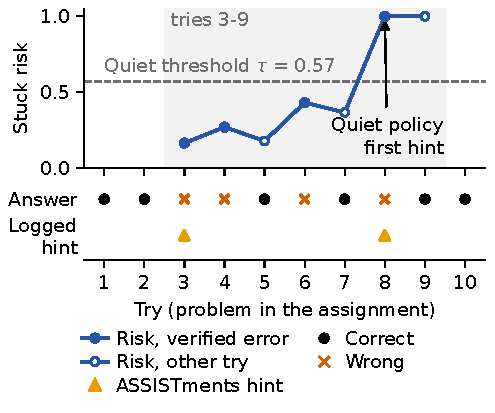
\includegraphics[width=\columnwidth]{figures/fig1_entanglement.pdf}
\caption{TODO caption: one validation sequence (selection rule in FIGURES.md): stuck risk, ARIA's decision points and first Quiet hint, and ASSISTments' own logged hints in the same window.}
\label{fig:entanglement}
\end{figure}

\section{Policy and Reporting Table}
% TODO: the abstention policy (risk >= tau at a verified error, one hint per problem set, three settings) and the CALE-AI reporting table.

% CALE-AI reporting table (the eight fields in the call). Filled from repository facts; "TODO" marks anything not settled in the repo.
% Sources: aria_pace/SPEC.md (Amendments 1, 2, 6, 7), docs/aria_pace/DATA.md, docs/aria_pace/PILOT_PROTOCOL.md, docs/cale/RESULTS_CALE.md (E3, E5-E8, E10).
\begin{table}[t]
\centering
\small
\setlength{\tabcolsep}{3pt}
\begin{tabular}{p{0.27\columnwidth}p{0.68\columnwidth}}
\toprule
Field & This work \\
\midrule
Intervention & One unsolicited hint per problem set from ARIA, given after a wrong first answer at tries 3--9 when the calibrated BKT stuck risk is $\ge\tau$ (Quiet 0.57, Balanced 0.19, Supportive 0.09). \\
Comparison condition & Offline: always-help, $n$-wrong-in-a-row rules, a random policy matched to the hint rate, PFA, and a logistic risk head. Planned trial: no ARIA hint at a decision point (usual ASSISTments support), randomized with probability 0.5. \\
Target population & ASSISTments 2009--10 skill-builder students (math). Grade level is not stated in the dataset. TODO: the planned trial population (grades, schools). \\
Human outcomes & None measured. The replay reports log-defined proxies (hints per student, missed help on the logged stuck label). Planned proximal outcome: correct first answer on the next problem. \\
Methodology & Pre-registered offline replay with a single locked test evaluation, 5-fold cross-validation, a closed-loop simulation under assumed student responses, and a planned micro-randomized trial. \\
Time horizon & Within one problem set: tries 1--10, measured in opportunities (no wall-clock time in the logs). Trial: next problem (proximal). TODO: sessions per student in the trial. \\
Adaptation mechanism & Per-skill BKT updated after every answer gives a stuck risk, which is Platt-calibrated and thresholded. Parameters and thresholds are frozen; there is no online learning. \\
Possible unintended effects & Missed help when wrong answers are hint requests (E3); students who already received ASSISTments hints (E5); uneven benefit across skills (E6); frustration or disengagement from withheld help (not measured). TODO: equity across student groups (no demographics in the data). \\
\bottomrule
\end{tabular}
\caption{CALE-AI reporting summary.}
\label{tab:reporting}
\end{table}


\section{Method}
% TODO: data (ASSISTments 2009-10), stuck label, BKT/PFA/risk head, Platt calibration, threshold choice by cost J, what was pre-registered.

\section{Evaluation Protocol}
% TODO: student split and locked test, 5-fold CV, metrics (hints per student, reduction vs always-help, missed help), baselines, bootstrap intervals, labels (locked-test / CV / validation / exploratory).

\section{Results}
% TODO: main table (locked test and CV side by side), trade-off curve, DKT/SAKT not promoted, A7 mastery definitions, E3/E4/E9.

% Generated by scripts/cale/paper_numbers.py from numbers.json (values via numbers.tex macros). Do not edit by hand.
\begin{table*}[t]
\centering
\small
\setlength{\tabcolsep}{4pt}
\begin{tabular}{lcccccc}
\toprule
 & \multicolumn{3}{c}{Locked 2009 test (\TestStudents{} students)} & \multicolumn{3}{c}{5-fold CV, held out (\CVStudents{} students)} \\
\cmidrule(lr){2-4}\cmidrule(lr){5-7}
Policy & Hints/student & Reduction (\%) & Missed help (\%) & Hints/student & Reduction (\%) & Missed help (\%) \\
\midrule
BKT Quiet ($\tau$ 0.57) & \QuietTestHints{\scriptsize\,\QuietTestHintsCI} & \QuietTestReduction & \QuietTestMissed{\scriptsize\,\QuietTestMissedCI} & \QuietCVHints{\scriptsize\,\QuietCVHintsCI} & \QuietCVReduction{\scriptsize\,\QuietCVReductionCI} & \QuietCVMissed{\scriptsize\,\QuietCVMissedCI} \\
BKT Balanced ($\tau$ 0.19) & \BalancedTestHints{\scriptsize\,\BalancedTestHintsCI} & \BalancedTestReduction & \BalancedTestMissed{\scriptsize\,\BalancedTestMissedCI} & \BalancedCVHints{\scriptsize\,\BalancedCVHintsCI} & \BalancedCVReduction{\scriptsize\,\BalancedCVReductionCI} & \BalancedCVMissed{\scriptsize\,\BalancedCVMissedCI} \\
BKT Supportive ($\tau$ 0.09) & \SupportiveTestHints{\scriptsize\,\SupportiveTestHintsCI} & \SupportiveTestReduction & \SupportiveTestMissed{\scriptsize\,\SupportiveTestMissedCI} & \SupportiveCVHints{\scriptsize\,\SupportiveCVHintsCI} & \SupportiveCVReduction{\scriptsize\,\SupportiveCVReductionCI} & \SupportiveCVMissed{\scriptsize\,\SupportiveCVMissedCI} \\
\midrule
Always-help & \AlwaysHelpTestHints{\scriptsize\,\AlwaysHelpTestHintsCI} & \AlwaysHelpTestReduction & \AlwaysHelpTestMissed{\scriptsize\,\AlwaysHelpTestMissedCI} & \AlwaysHelpCVHints{\scriptsize\,\AlwaysHelpCVHintsCI} & \AlwaysHelpCVReduction{\scriptsize\,\AlwaysHelpCVReductionCI} & \AlwaysHelpCVMissed{\scriptsize\,\AlwaysHelpCVMissedCI} \\
Two-wrong rule (tuned) & \TwoWrongTestHints{\scriptsize\,\TwoWrongTestHintsCI} & \TwoWrongTestReduction & \TwoWrongTestMissed{\scriptsize\,\TwoWrongTestMissedCI} & \TwoWrongCVHints{\scriptsize\,\TwoWrongCVHintsCI} & \TwoWrongCVReduction{\scriptsize\,\TwoWrongCVReductionCI} & \TwoWrongCVMissed{\scriptsize\,\TwoWrongCVMissedCI} \\
Three-wrong rule (untuned) & \ThreeWrongTestHints{\scriptsize\,\ThreeWrongTestHintsCI} & \ThreeWrongTestReduction & \ThreeWrongTestMissed{\scriptsize\,\ThreeWrongTestMissedCI} & \ThreeWrongCVHints{\scriptsize\,\ThreeWrongCVHintsCI} & \ThreeWrongCVReduction{\scriptsize\,\ThreeWrongCVReductionCI} & \ThreeWrongCVMissed{\scriptsize\,\ThreeWrongCVMissedCI} \\
Random, matched to Quiet & \RandomTestHints{\scriptsize\,\RandomTestHintsCI} & \RandomTestReduction & \RandomTestMissed{\scriptsize\,\RandomTestMissedCI} & \RandomCVHints{\scriptsize\,\RandomCVHintsCI} & \RandomCVReduction{\scriptsize\,\RandomCVReductionCI} & \RandomCVMissed{\scriptsize\,\RandomCVMissedCI} \\
PFA ($\tau$ 0.46) & \PFATestHints{\scriptsize\,\PFATestHintsCI} & \PFATestReduction & \PFATestMissed{\scriptsize\,\PFATestMissedCI} & \PFACVHints{\scriptsize\,\PFACVHintsCI} & \PFACVReduction{\scriptsize\,\PFACVReductionCI} & \PFACVMissed{\scriptsize\,\PFACVMissedCI} \\
Risk head ($\tau$ 0.55) & \RiskHeadTestHints{\scriptsize\,\RiskHeadTestHintsCI} & \RiskHeadTestReduction & \RiskHeadTestMissed{\scriptsize\,\RiskHeadTestMissedCI} & \RiskHeadCVHints{\scriptsize\,\RiskHeadCVHintsCI} & \RiskHeadCVReduction{\scriptsize\,\RiskHeadCVReductionCI} & \RiskHeadCVMissed{\scriptsize\,\RiskHeadCVMissedCI} \\
\bottomrule
\end{tabular}
\caption{Main results. Test: the single locked evaluation with thresholds frozen on validation; reductions on test have no interval in the result file. CV: the same frozen thresholds applied to per-fold calibrated risk on held-out folds (post hoc, CALE E1). Missed help = stuck sequences with a help opportunity that received no hint before try 10 (test $N=\TestStuckOpp$, CV $N=\CVStuckOpp$). Baselines, PFA and the risk head are at the Quiet setting; the tuned rule for Balanced and Supportive is always-help. Brackets: 95\% student-bootstrap intervals.}
\label{tab:main}
\end{table*}


\begin{figure}[t]
\centering
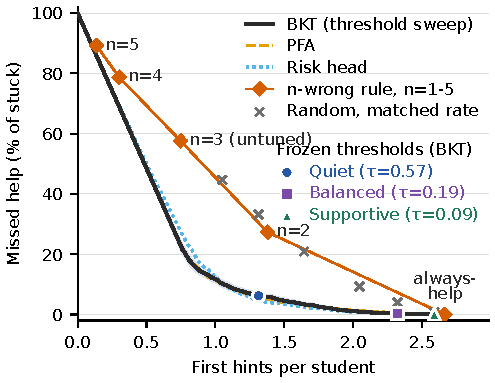
\includegraphics[width=\columnwidth]{../../aria_pace/results_cale/figures/e1_tradeoff.pdf}
\caption{TODO caption: trade-off between first hints per student and missed help on CV held-out students (CALE E1).}
\label{fig:tradeoff}
\end{figure}

\section{What Replay Cannot Tell Us}
% TODO: entanglement with logged hints (E5, E7, E8), the closed-loop simulation and its flip point (robust evaluation matrix), no learning or affect outcome.

% Generated by scripts/cale/paper_numbers.py from aria_pace/results/closed_loop_sensitivity.json (A6). Do not edit by hand.
\begin{table}[t]
\centering
\small
\setlength{\tabcolsep}{3.5pt}
\begin{tabular}{lcccc}
\toprule
Assumed & \multicolumn{3}{c}{Grid points (of 20)} & $\Delta J$ per sequence \\
\cmidrule(lr){2-4}
$p_{\mathrm{stuck}}$ & Quiet & Tie & Always & (Quiet $-$ always) \\
\midrule
0 & 20 & 0 & 0 & $-0.60$ to $-0.52$ \\
0.05 & 20 & 0 & 0 & $-0.29$ to $-0.21$ \\
0.1 & 0 & 5 & 15 & $+0.00$ to $+0.07$ \\
0.2 & 0 & 0 & 20 & $+0.56$ to $+0.62$ \\
0.3 & 0 & 0 & 20 & $+1.07$ to $+1.11$ \\
\bottomrule
\end{tabular}
\caption{Closed-loop simulation (A6; assumed simulated students, not evidence of effect): when does the Quiet policy ($\tau=0.57$) beat always-help? Rows: the assumed probability that a student left unaided after a wrong step abandons, the assumption that drives the sign. Each row pools 5 help-effect values (0--0.5) $\times$ 4 interruption-cost values (0--0.3). Quiet / Always: that policy has the lower cost $J$; tie: the 95\% interval of simulation noise includes 0. Quiet's advantage flips at $p_{\mathrm{stuck}}\approx\AsixSimQuietFlipMin$--\AsixSimQuietFlipMax. Supportive ($\tau=0.09$) makes the same decisions as always-help at every point.}
\label{tab:robust}
\end{table}


\section{Planned Micro-Randomized Trial}
% TODO: decision points, proximal outcome, randomization 0.5, base rate and sample sizes (E10), and the feasibility pilot.

\section{Limitations and Conclusion}
% TODO: single dataset and era, inferred first_action codes, logged label, no human outcomes, post hoc analyses; what the paper does and does not claim.

\bibliography{refs}

\end{document}
